\documentclass[10pt]{beamer}
\usepackage{xeCJK}
\usepackage[utf8]{inputenc}
% \usepackage{xeCJK} % Disabled to avoid Fandol font error
\usepackage{graphicx}
\usepackage {mathtools}
\usepackage[inkscapeformat=png]{svg}
\usepackage{utopia} %font utopia imported
\usetheme{CambridgeUS}
% \usepackage{fontspec}
\usepackage{svg}
\usepackage{tikz}
\usepackage{caption}
\usepackage{diagbox} 
\usepackage[absolute,overlay]{textpos}
\usepackage[table]{xcolor} % enables \rowcolor, \columncolor in tables
\usepackage{pifont} % for attention sign 
\usetikzlibrary{positioning,calc}
\usetikzlibrary{positioning,arrows.meta,calc}
% \usepackage{fourier}  % sans serif font
\renewcommand{\familydefault}{\sfdefault}
\usecolortheme{dolphin}
\usepackage[backend=biber,style=authoryear]{biblatex}
\addbibresource{bibliography.bib} % Ensure bibliography.bib exists and contains at least one entry with key 'example_reference'

% set colors to University of Kassel colours
\definecolor{myNewColorA}{RGB}{172,4,76}
\definecolor{myNewColorB}{RGB}{197,83,132}
\definecolor{myNewColorC}{RGB}{209,145,173}
\setbeamercolor*{palette primary}{bg=myNewColorC}
\setbeamercolor*{palette secondary}{bg=myNewColorB, fg = white}
\setbeamercolor*{palette tertiary}{bg=myNewColorA, fg = white}
\setbeamercolor*{titlelike}{fg=myNewColorA}
\setbeamercolor*{title}{bg=myNewColorA, fg = white}
\setbeamercolor*{item}{fg=myNewColorA}
\setbeamercolor*{caption name}{fg=myNewColorA}
\usefonttheme{professionalfonts}
\usepackage{hyperref}
\usepackage[printonlyused]{acronym}
% \usepackage[nolist]{acronym}    

% Progress bar in headline (fixed version)
\makeatletter
\setbeamertemplate{headline}{%
  \begin{tikzpicture}[remember picture,overlay]
    % Bar height
    \def\barheight{0.15cm}
    % Background bar (full width)
    \fill[myNewColorC] (current page.north west) rectangle 
                       ([yshift=-\barheight]current page.north east);
    % Progress bar (partial width)
    \fill[myNewColorA] (current page.north west) rectangle 
      ($ (current page.north west) + (\paperwidth*\insertframenumber/\inserttotalframenumber,-\barheight) $);
  \end{tikzpicture}%
  \vspace{0.2cm} % Space below the bar
}
\makeatother



%------------------------------------------------------------
% \titlegraphic{
\includegraphics[height=1.5cm]{images/Logo_Uni_Kassel.png}}
\titlegraphic{%
  
\includegraphics[height=1.5cm]{images/Finanzamt_Kassel.png}\hspace{0.5cm}%
  
\includegraphics[height=1.5cm]{images/Logo_Uni_Kassel}\hspace{0.5cm}%
  
\includegraphics[height=1.5cm]{images/partner-dhbw-450x238.png}%
}
\newcommand{\university}{University of Kassel}
\setbeamerfont{title}{size=\large}
\setbeamerfont{subtitle}{size=\small}
\setbeamerfont{author}{size=\small}
\setbeamerfont{date}{size=\small}
\setbeamerfont{institute}{size=\small}
% \setbeamerfont{instituteB}{size=\small}
\title[\university{}]{Conceptual Topic Aggregation (\acs{approachname})}
\subtitle{A Case Study on the \acs{dataset} Dataset}
\author[Klara M. Gutekunst]{\underline{Klara M. Gutekunst} \and Dominik Dürrschnabel \and Johannes Hirth \and Gerd Stumme}

\institute[klara.gutekunst@uni-kassel.de]{\university{}}
% \instituteB[KDE]{\inst{2}Knowledge and Data Engineering Group
% Department of Electrical Engineering and Computer Science
% Interdisciplinary Research Center for Information System Design
% University of Kassel}
\date[\today]
{\today}

%------------------------------------------------------------
%This block of commands puts the table of contents at the 
%beginning of each section and highlights the current section:
%\AtBeginSection[]
%{
%  \begin{frame}
%    \frametitle{Contents}
%    \tableofcontents[currentsection]
%  \end{frame}
%}
\AtBeginSection[]{
  \begin{frame}
  \vfill
  \centering
  \begin{beamercolorbox}[sep=8pt,center,shadow=true,rounded=true]{title}
    \usebeamerfont{title}\insertsectionhead\par%
  \end{beamercolorbox}
  \vfill
  \end{frame}
}
%------------------------------------------------------------

\begin{document}
% \setmainfont{Crimson Pro}

%The next statement creates the title page.
\frame{\titlepage}
\begin{frame}
\frametitle{Contents}
\tableofcontents
\end{frame}
%------------------------------------------------------------
\newcommand{\FormalConceptGraph}{%
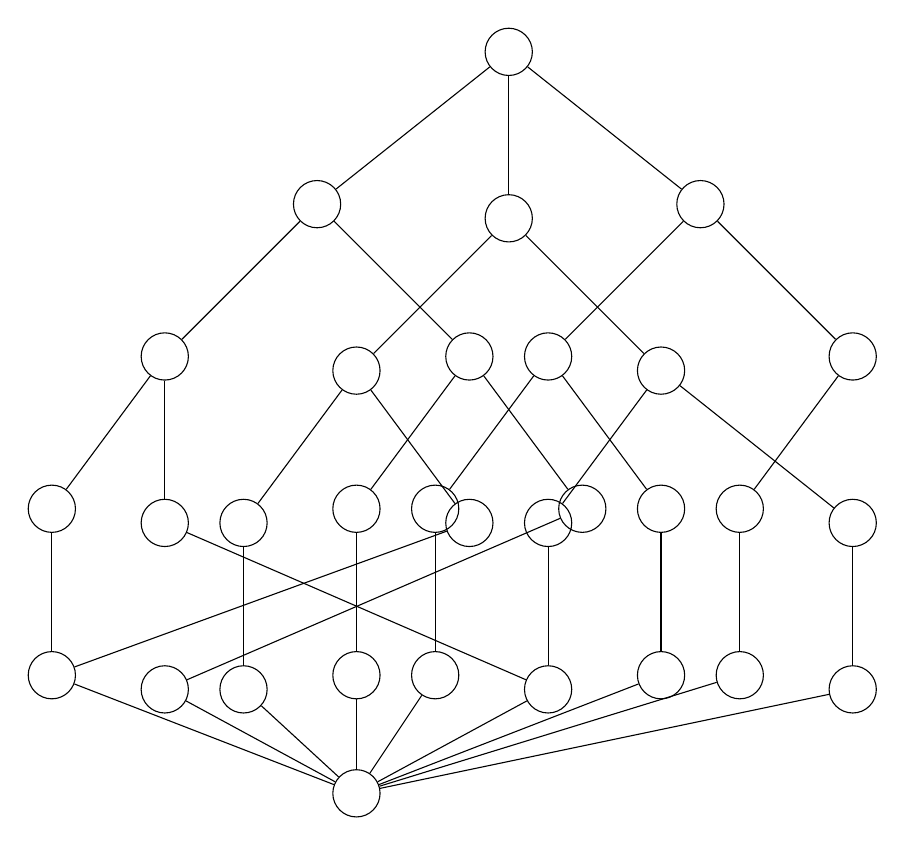
\begin{tikzpicture}[
    concept/.style={
        circle, draw, minimum size=6mm, inner sep=1mm
    },
    level distance=15mm
]
    
    % Layer 0 (top)
    \node[concept] (n0) {};

    % Layer 1
    \node[concept, below left=15mm and 20mm of n0] (n1) {};
    \node[concept, below=15mm of n0] (n2) {};
    \node[concept, below right=15mm and 20mm of n0] (n3) {};

    % Layer 2
    \node[concept, below left=15mm and 15mm of n1] (n4) {};
    \node[concept, below right=15mm and 15mm of n1] (n5) {};
    \node[concept, below left=15mm and 15mm of n2] (n6) {};
    \node[concept, below right=15mm and 15mm of n2] (n7) {};
    \node[concept, below left=15mm and 15mm of n3] (n8) {};
    \node[concept, below right=15mm and 15mm of n3] (n9) {};

    % Layer 3
    \node[concept, below left=15mm and 10mm of n4] (n10) {};
    \node[concept, below=15mm and 10mm of n4] (n11) {};
    \node[concept, below left=15mm and 10mm of n5] (n12) {};
    \node[concept, below right=15mm and 10mm of n5] (n13) {};
    \node[concept, below left=15mm and 10mm of n6] (n14) {};
    \node[concept, below right=15mm and 10mm of n6] (n15) {};
    \node[concept, below left=15mm and 10mm of n7] (n16) {};
    \node[concept, below=15mm and 10mm of n9] (n17) {};
    \node[concept, below left=15mm and 10mm of n8] (n18) {};
    \node[concept, below right=15mm and 10mm of n8] (n19) {};
    \node[concept, below left=15mm and 10mm of n9] (n20) {};

    % Layer 4 (bottom)
    \node[concept, below=15mm of n10] (n22) {};
    \node[concept, below=15mm of n12] (n23) {};
    \node[concept, below=15mm of n14] (n24) {};
    \node[concept, below=15mm of n16] (n25) {};
    \node[concept, below=15mm of n18] (n26) {};
    \node[concept, below=15mm of n20] (n27) {};
    \node[concept, below=15mm of n11] (n28) {};
    \node[concept, below=15mm of n17] (n29) {};
    \node[concept, below=15mm of n19] (n30) {};

    % Single bottom node
    \node[concept] (n31) at ($ (n22)!0.5!(n30) + (0,-15mm) $) {};
    % \node[concept] (n31) at ($(n22)!0.5!(n30) - (0,15mm)$) {};
    % \node[concept, below=15mm of $(n22)!0.5!(n30)$] (n31) {};

    % Draw downward edges only
    \foreach \from/\to in {
        n0/n1, n0/n2, n0/n3,
        n1/n4, n1/n5, n2/n6, n2/n7, n3/n8, n3/n9,
        n4/n10, n4/n11, n5/n12, n5/n13, n6/n14, n6/n15, n7/n16, n7/n17, n8/n18, n8/n19, n9/n20, 
        n10/n22, n11/n25, n12/n23, n13/n28, n14/n24, n15/n22, n16/n25, n17/n29, n18/n26, n19/n30, n20/n27}
    {
        \draw (\from) -- (\to);
    }

    % Connect all bottom layer nodes to the single bottom node
    \foreach \n in {n22,n23,n24,n25,n26,n27,n28,n29,n30}
    {
        \draw (\n) -- (n31);
    }

\end{tikzpicture}%
}


\newcommand{\FormalConceptGraphColoured}{%
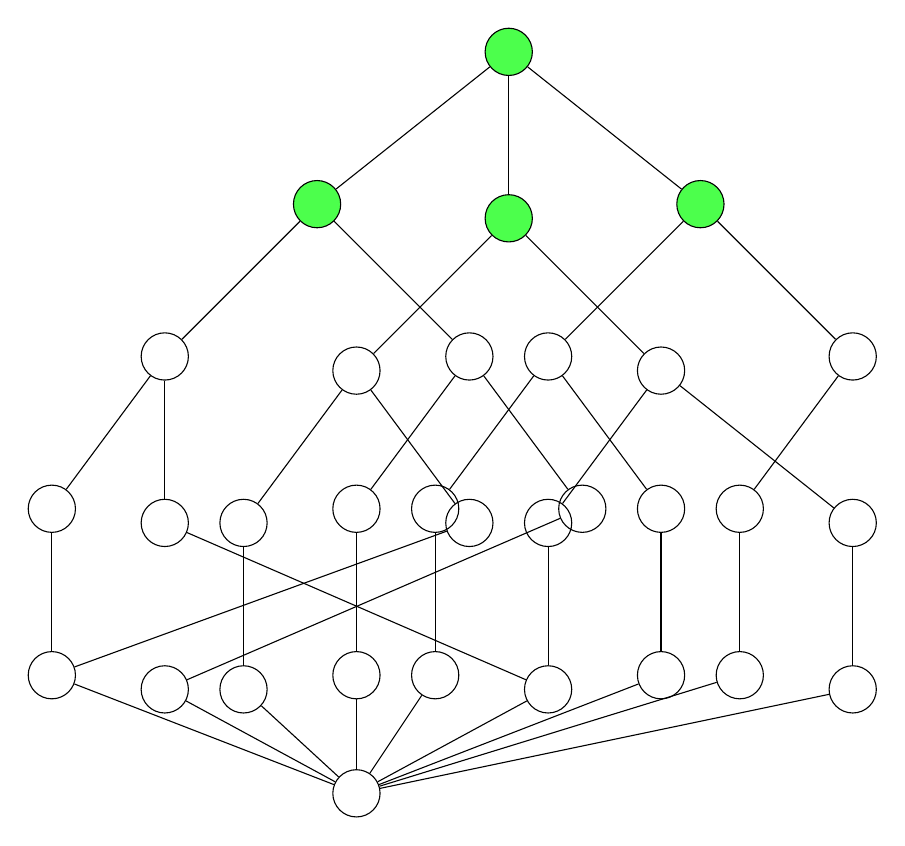
\begin{tikzpicture}[
    concept/.style={
        circle, draw, minimum size=6mm, inner sep=1mm
    },
    level distance=15mm
]

% Layer 0
\node[concept, fill=green!70] (n0) {};

% Layer 1
\node[concept, below left=15mm and 20mm of n0, fill=green!70] (n1) {};
\node[concept, below=15mm of n0, fill=green!70] (n2) {};
\node[concept, below right=15mm and 20mm of n0, fill=green!70] (n3) {};

   % Layer 2
    \node[concept, below left=15mm and 15mm of n1] (n4) {};
    \node[concept, below right=15mm and 15mm of n1] (n5) {};
    \node[concept, below left=15mm and 15mm of n2] (n6) {};
    \node[concept, below right=15mm and 15mm of n2] (n7) {};
    \node[concept, below left=15mm and 15mm of n3] (n8) {};
    \node[concept, below right=15mm and 15mm of n3] (n9) {};

    % Layer 3
    \node[concept, below left=15mm and 10mm of n4] (n10) {};
    \node[concept, below=15mm and 10mm of n4] (n11) {};
    \node[concept, below left=15mm and 10mm of n5] (n12) {};
    \node[concept, below right=15mm and 10mm of n5] (n13) {};
    \node[concept, below left=15mm and 10mm of n6] (n14) {};
    \node[concept, below right=15mm and 10mm of n6] (n15) {};
    \node[concept, below left=15mm and 10mm of n7] (n16) {};
    \node[concept, below=15mm and 10mm of n9] (n17) {};
    \node[concept, below left=15mm and 10mm of n8] (n18) {};
    \node[concept, below right=15mm and 10mm of n8] (n19) {};
    \node[concept, below left=15mm and 10mm of n9] (n20) {};

    % Layer 4 (bottom)
    \node[concept, below=15mm of n10] (n22) {};
    \node[concept, below=15mm of n12] (n23) {};
    \node[concept, below=15mm of n14] (n24) {};
    \node[concept, below=15mm of n16] (n25) {};
    \node[concept, below=15mm of n18] (n26) {};
    \node[concept, below=15mm of n20] (n27) {};
    \node[concept, below=15mm of n11] (n28) {};
    \node[concept, below=15mm of n17] (n29) {};
    \node[concept, below=15mm of n19] (n30) {};

    % Single bottom node
    \node[concept] (n31) at ($ (n22)!0.5!(n30) + (0,-15mm) $) {};
    % \node[concept] (n31) at ($(n22)!0.5!(n30) - (0,15mm)$) {};
    % \node[concept, below=15mm of $(n22)!0.5!(n30)$] (n31) {};

    % Draw downward edges only
    \foreach \from/\to in {
        n0/n1, n0/n2, n0/n3,
        n1/n4, n1/n5, n2/n6, n2/n7, n3/n8, n3/n9,
        n4/n10, n4/n11, n5/n12, n5/n13, n6/n14, n6/n15, n7/n16, n7/n17, n8/n18, n8/n19, n9/n20, 
        n10/n22, n11/n25, n12/n23, n13/n28, n14/n24, n15/n22, n16/n25, n17/n29, n18/n26, n19/n30, n20/n27}
    {
        \draw (\from) -- (\to);
    }

    % Connect all bottom layer nodes to the single bottom node
    \foreach \n in {n22,n23,n24,n25,n26,n27,n28,n29,n30}
    {
        \draw (\n) -- (n31);
    }


\end{tikzpicture}%
}

\section{Motivation}
\begin{frame}{Motivation}
    \only<1>{
        \begin{figure}
            \includesvg[width=\linewidth]{images/steps/overview.svg}
        \end{figure}
    } 
    \only<2>{
        \begin{figure}
            \includesvg[width=\linewidth]{images/steps/overview_step1.svg}
        \end{figure}
    } 
    \only<3>{
        \begin{figure}
            \includesvg[width=\linewidth]{images/motivation/motivation1.svg}
        \end{figure}
    }
    \only<4>{
        \begin{figure}
            \includesvg[width=\linewidth]{images/motivation/motivation2.svg}
        \end{figure}
    }
    \only<5>{
        \begin{figure}
            \includesvg[width=\linewidth]{images/motivation/motivation3.svg}
        \end{figure}
    }
\end{frame}

\begin{frame}{Motivation} 
    \begin{columns}
        \begin{column}{0.8\textwidth}
            \begin{alertblock}{Problem} 
            Employees at the tax office often lack prior knowledge about the contents of the data before starting exploration.
            \end{alertblock}

            \visible<2->{What is our objective?\\}
            \visible<3->{$\rightarrow$ \textbf{Gain an initial understanding of the data.}}
        \end{column}
        \begin{column}{0.18\textwidth}
            \begin{figure}
                \centering
                
\includegraphics[width=0.7\textwidth]{images/motivation/tax.png}
            \end{figure}
        \end{column}
    \end{columns}
\end{frame}


\begin{frame}{Motivation} 
    \begin{exampleblock}{Objective} 
    Gain an initial understanding of the data.
    \end{exampleblock}

    \visible<2->{\textbf{Challenges:}}
    \begin{itemize}
        \item[\ding{55}]<3-> Lack of labeled data for supervised training
        \item[\ding{55}]<4-> Diverse data formats and structures
    \end{itemize}

    \visible<5->{How did we tackle these problems?}
    \begin{itemize}
        \item[\ding{51}]<6-> Fully unsupervised analysis pipeline
        \item[\ding{51}]<7-> Handles multiple languages and file types
    \end{itemize}
\end{frame}
\section{Dataset}

\begin{frame}{Everything You Need To Know Ever\footnote{\url{https://archive.org/details/ETYNTKE} (29.01.2025)}}
    \begin{columns}[T] % align top
        \begin{column}{0.6\textwidth}
             \begin{itemize}
                \item Approx. 101 GB 
                \item Images, text documents, and other file types
                \item Malformed files
                \item Uploaded in 2015
                \item Topics include politics, weaponry, and Computer Science
                \item Hierarchical organization into directories
            \end{itemize}
        \end{column}

        \begin{column}{0.3\textwidth}
            \begin{figure}
                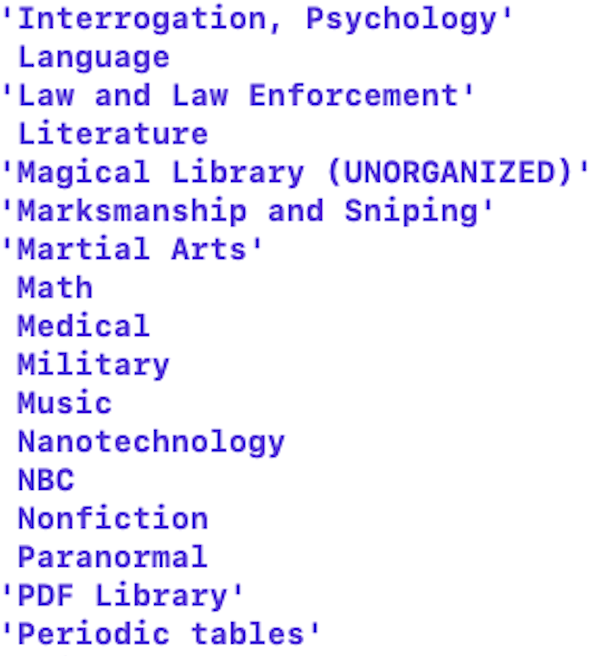
\includegraphics[width=\linewidth]{images/screenshot_data.png}
                \caption{Subset of top-level directories in the ETYNTKE dataset.} % replaces \caption
            \end{figure}
   
        \end{column}
    \end{columns}
\end{frame}



% \section{Mathematical Foundations}



\section{Prior Work}

\begin{frame}{Selection of Prior Work}
    Assuming we work on data structured in directories.
    \begin{itemize}
        \item<2-> Topic models (LDA, BERTopic, and Top2Vec)
        \begin{itemize}
            \item[$\checkmark$]<3-> Topic identification
            \item[$\times$]<3-> Do not leverage intrinsic hierarchical structure of documents
        \end{itemize}

        \item<4-> \acs{fca} on Twitter data~\cite{twitter_fca_2016}
        \begin{itemize}
            \item[$\checkmark$]<5-> Support frequency thresholds 
            \item[$\times$]<5-> Term frequency rather than semantics
        \end{itemize}
      
    \end{itemize}
\end{frame}



\begin{frame}{Prior Work}
    
    \begin{itemize}
   
        \item<1-> Representation of document-topic relations using a concept lattice~\cite{topic_modeling_2024}
        \begin{itemize}
            \item[$\checkmark$]<3-> Hierarchical representation
            \item[$\checkmark$]<3-> Excluding low support items
            \item[$\times$]<3-> Homogeneous dataset (academic papers on Machine Learning)
            \item[$\times$]<3-> Exclusively textual data
            \item[$\times$]<3-> Lacks ability to aggregate information 
        \end{itemize}
    \end{itemize}


\only<2->{%
    \centering
    \begin{minipage}{\textwidth}
        % --- Document-topic relation ---
        \begin{minipage}{0.48\textwidth}
            \centering
            \captionof{table}{Document-topic relation}
            \label{tab:doc-topic}
            \resizebox{\linewidth}{!}{%
                \begin{tabular}{|c|c|c|c|c|}
                    \hline
                    \diagbox{Documents}{Topics} & $t_1$ & $t_2$ & $\cdots$ & $t_n$ \\ \hline
                    $d_1$ & $w_{1,1}$ & $w_{1,2}$ & $\cdots$ & $w_{1,n}$ \\ \hline
                    $d_2$ & $w_{2,1}$ & $w_{2,2}$ & $\cdots$ & $w_{2,n}$ \\ \hline
                    $\vdots$ & $\vdots$ & $\vdots$ & $\ddots$ & $\vdots$ \\ \hline
                    $d_l$ & $w_{l,1}$ & $w_{l,2}$ & $\cdots$ & $w_{l,n}$ \\ \hline
                \end{tabular}
            }
        \end{minipage}%
        \hfill
        % --- Term-topic relation ---
        \begin{minipage}{0.48\textwidth}
            \centering
            \captionof{table}{Term-topic relation}
            \label{tab:term-topic}
            \resizebox{\linewidth}{!}{%
                \begin{tabular}{|c|c|c|c|c|}
                    \hline
                    \diagbox{Terms}{Topics} & $t_1$ & $t_2$ & $\cdots$ & $t_n$ \\ \hline
                    $s_1$ & $\hat{w}_{1,1}$ & $\hat{w}_{1,2}$ & $\cdots$ & $\hat{w}_{1,n}$ \\ \hline
                    $s_2$ & $\hat{w}_{2,1}$ & $\hat{w}_{2,2}$ & $\cdots$ & $\hat{w}_{2,n}$ \\ \hline
                    $\vdots$ & $\vdots$ & $\vdots$ & $\ddots$ & $\vdots$ \\ \hline
                    $s_l$ & $\hat{w}_{l,1}$ & $\hat{w}_{l,2}$ & $\cdots$ & $\hat{w}_{l,n}$ \\ \hline
                \end{tabular}
            }
        \end{minipage}
    \end{minipage}%
}


\end{frame}



\section{Our Approach}
\begin{frame}{Our Approach}
    \begin{description}
    \item[\acs{approachname}] \acl{approachname}
    \end{description}
    
    \only<1>{
        \begin{figure}[htbp]
        \centering
            
\includegraphics[height=0.6\textheight]{images/DALLE_2025_02_21_fat_cat.png}
        \label{fig:fat_cat}
    \end{figure}
    Image generated by DALLE (February 21, 2025)
    }

    \only<2->{
        \begin{figure}[htbp]
        \centering
        \scalebox{0.9}{
            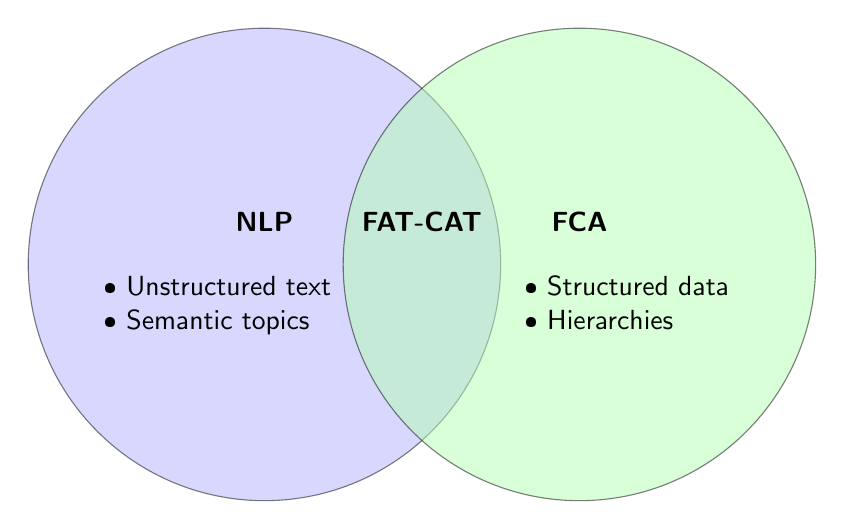
\begin{tikzpicture}
                 % Draw circles
                \draw[fill=blue!30, opacity=0.5] (-2,0) circle (3);
                \draw[fill=green!30, opacity=0.5] (2,0) circle (3);

                % Labels above circles
                \node[above] at (-2,0.3) {\textbf{NLP}};
                \node[above] at (2,0.3) {\textbf{FCA}};
                \node[above] at (0,0.3) {\textbf{FAT-CAT}};

                % NLP-only contributions (inside left circle, lower)
                \node[align=left] at (-2.6,-0.7) {
                    \textbullet\ Unstructured text\\
                    \textbullet\ Semantic topics\\
                    % \textbullet\ Statistical\\
                };

                % FCA-only contributions (inside right circle, lower)
                \node[align=left] at (2.6,-0.7) {
                    \textbullet\ Structured data\\
                    \textbullet\ Hierarchies\\
                    % \textbullet\ Deductive reasoning\\
                };
            \end{tikzpicture}
        }
        \label{fig:venn_nlp_fca}
    \end{figure}
    }

\end{frame}

\begin{frame}{Our Approach}
    \begin{description}
    \item[\acs{approachname}] \acl{approachname}
    \end{description}

    Our contributions:
    \begin{itemize}
        \uncover<2->{\item Open-source\footnote{\url{https://github.com/KlaraGtknst/text_topic} (29.01.2025) \&\\ \url{https://github.com/KlaraGtknst/clj_exploration_leaks} (29.01.2025)}}
        \uncover<3->{\item Minimal training requirements}
        \uncover<4->{\item Non-textual data} % \item[\rightarrowfill]
        \uncover<5->{\item Information aggregation across directories}       
    \end{itemize}
\end{frame}
\section{Results}
\begin{frame}{Topics}
    \begin{itemize}
        \item 50 words per topic
        \item Multi-lingual
    \end{itemize}
    \visible<2->{
        \begin{table}[H]
        \centering
        \caption{Subset of translated topic IDs and their top 5 descriptive words for the directory-topic concept lattice.}
        \label{tab:dir_topic_topics2terms}
        \resizebox{\textwidth}{!}{%
            \begin{tabular}{|
                    >{\columncolor[HTML]{D4D4D4}}l |l|l|l|l|l|}
                \hline
                \rowcolor[HTML]{D4D4D4}
                \textbf{Topic ID} & \multicolumn{5}{c|}{\textbf{Topic Words}}                                                                   \\ \hline
                \textbf{34}       & gun                                       & weapons      & rifles          & pistol         & firearm       \\ \hline
                \textbf{36}       & terminological                            & nonverbal    & linguist        & codeword       & longtext      \\ \hline
                \textbf{54}       & microelectron                             & microkernels & microparticle   & microphysics   & microcosmic   \\ \hline
                \textbf{56}       & pythonpath                                & pythonmac    & python\_version & python\_object & pythonpowered \\ \hline
                \textbf{58}       & nuclear                                   & hazardous    & explosive       & nanotoxicity   & chernobyl     \\ \hline
                \textbf{94}       & project                                   & fundraiser   & donation        & volunteering   & charity       \\ \hline
            \end{tabular}%
            }
        \end{table}
        }
\end{frame}

\begin{frame}{Directory-Topic Concept Lattice}

    \begin{figure}[t]
        \centering
        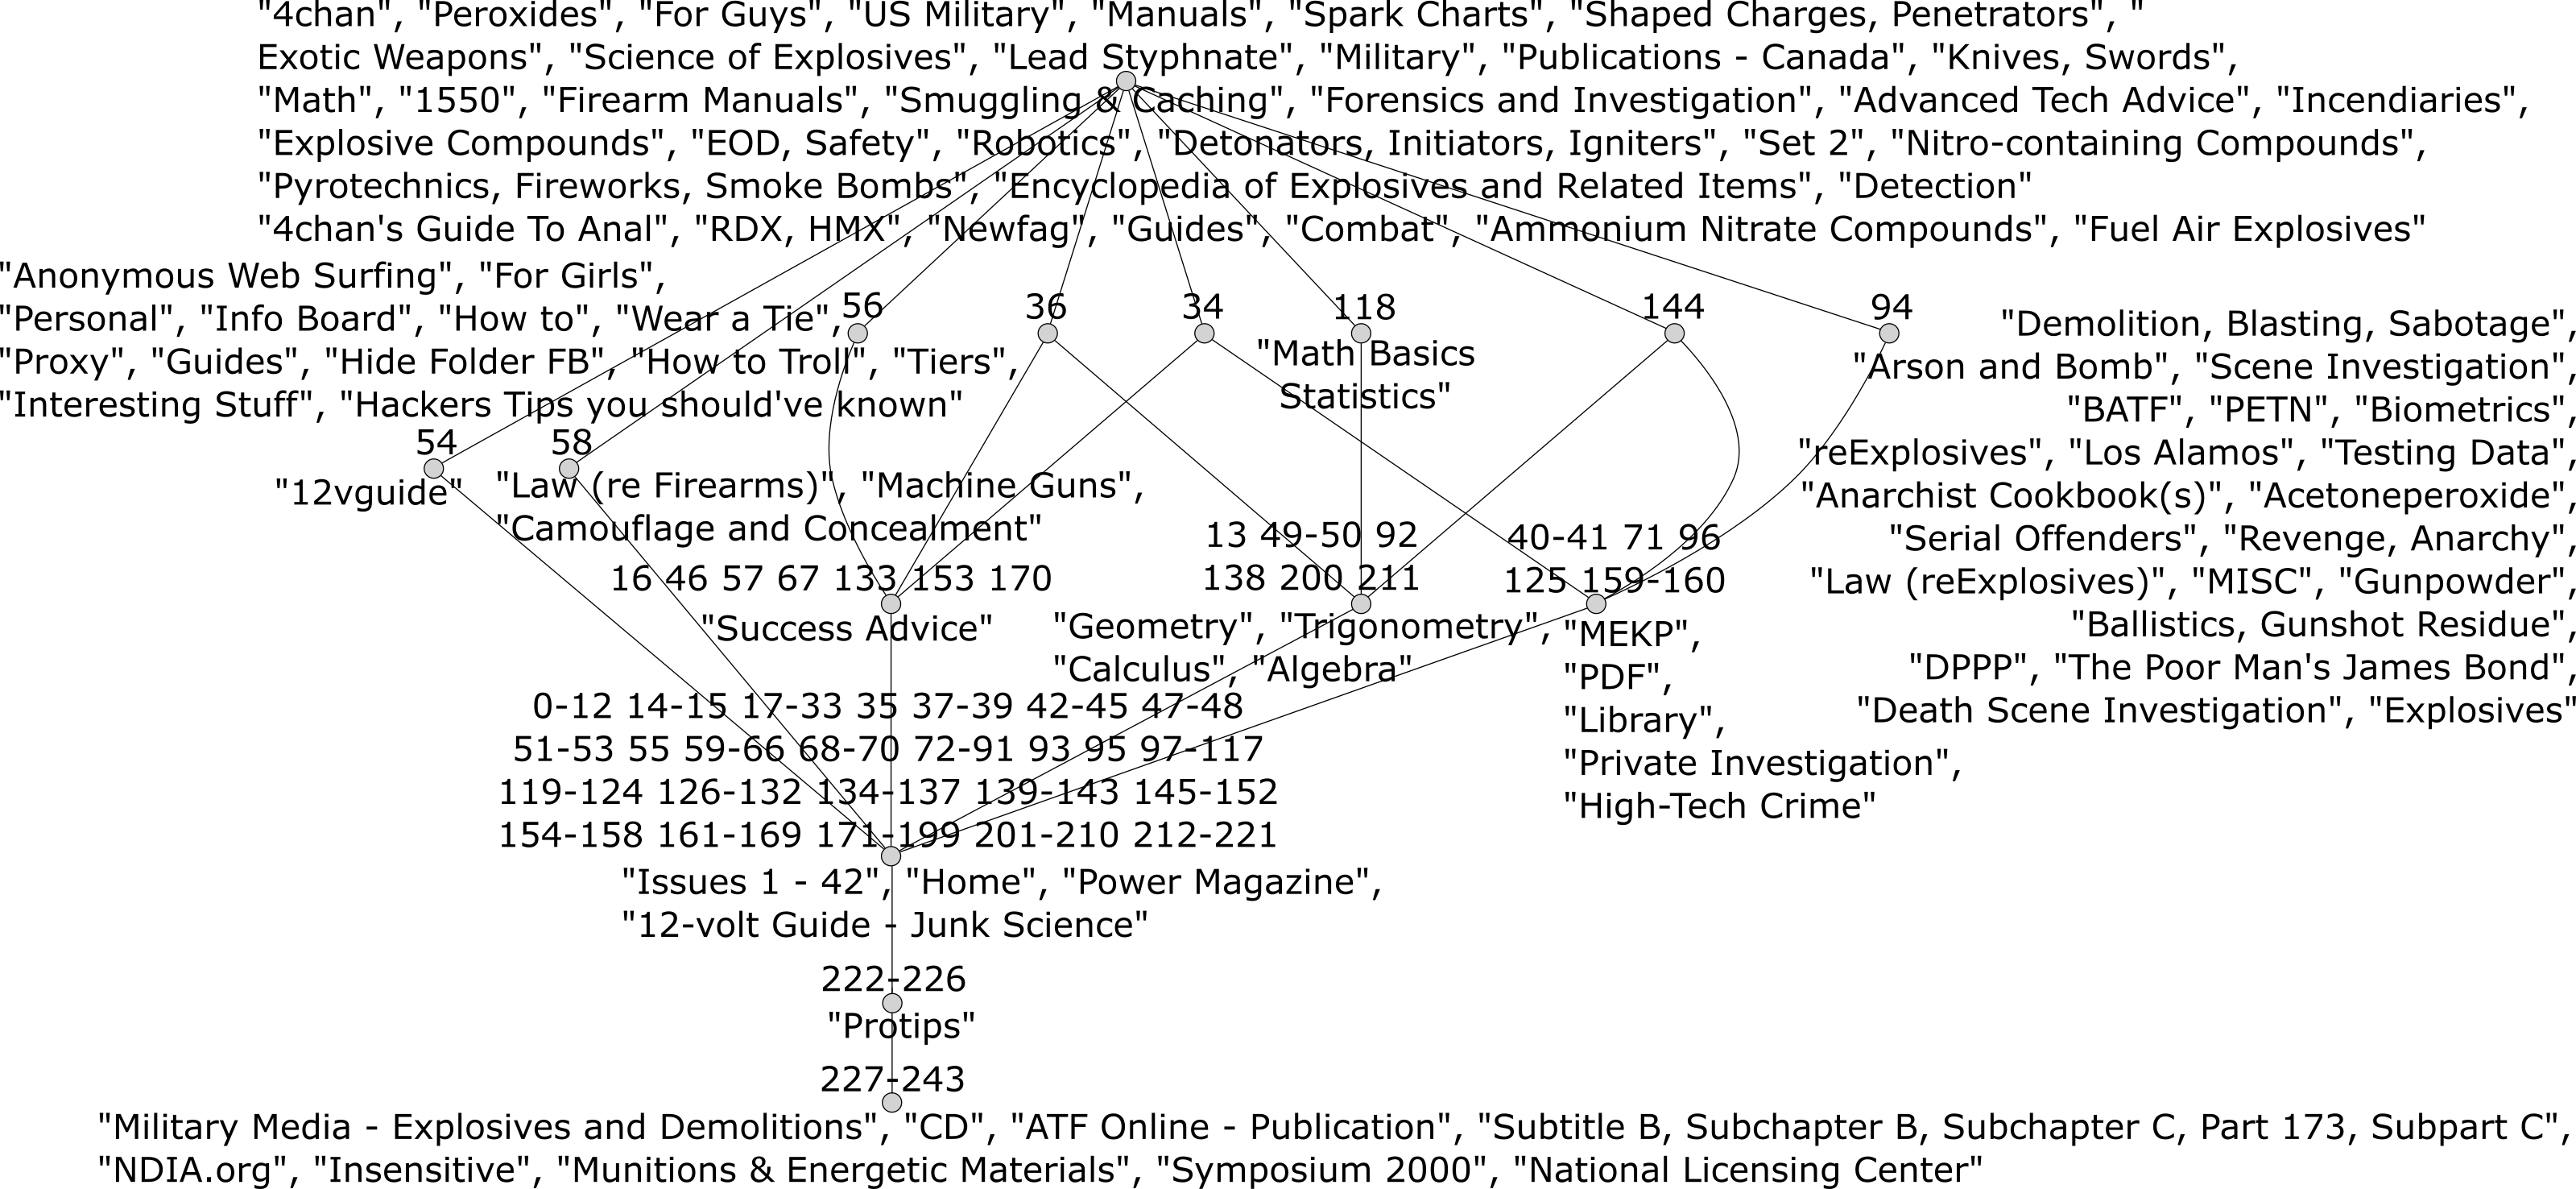
\includegraphics[width=\textwidth]{images/fca_graph_across_dirs_02_03_25_altered3.png}
        \caption{\ac{dataset} directory-topic concept lattice.
            The text entries below the nodes represent directory names, number above nodes denote topic IDs.
        }
        \label{fig:fca_across_dirs}
    \end{figure}
    
\end{frame}

\begin{frame}{Directory-Topic Concept Lattice}

    \begin{itemize}
        \item "Common to specific": Topics propagate downwards 
        \item<2-> Motifs
        \item<3-> Majority of bottom nodes is subdirectory
        \item<4-> Lower nodes introduce philosophical topics
    \end{itemize}

    \visible<2->{
        \begin{definition}
            A motif is a statistically significant subgraph or pattern \cite{hirth_ordinal_2024}.
        \end{definition}
    }
\end{frame}
\begin{frame}{What I've learnt...}
    
\end{frame}
\section{Conclusion}
\begin{frame}{Conclusion}
    \begin{exampleblock}{Objective} 
    Gain an initial understanding of the data.
    \end{exampleblock}
    \begin{itemize}
        \item[\textcolor{green}{+}]<2-> Dataset exploration without manual inspection
        \item[\textcolor{green}{+}]<3-> Semantic relationship of directories
        \item[\textcolor{red}{-}]<4-> Unintuitive for inexperienced users
        \item[\textcolor{red}{-}]<5-> Numerical topic representation
    \end{itemize}
    \only<2>{
        \begin{figure}
            \includesvg[width=\textwidth]{images/steps/overview_step3.svg}
        \end{figure}
    }
    \only<3>{
        \begin{figure}
            \centering
            \includesvg[width=0.65\textwidth]{images/steps_detail/topic_modeling_fca_2rows_step5.svg}
        \end{figure}
    }
    \only<4>{
        \begin{figure}[t]
            \centering
            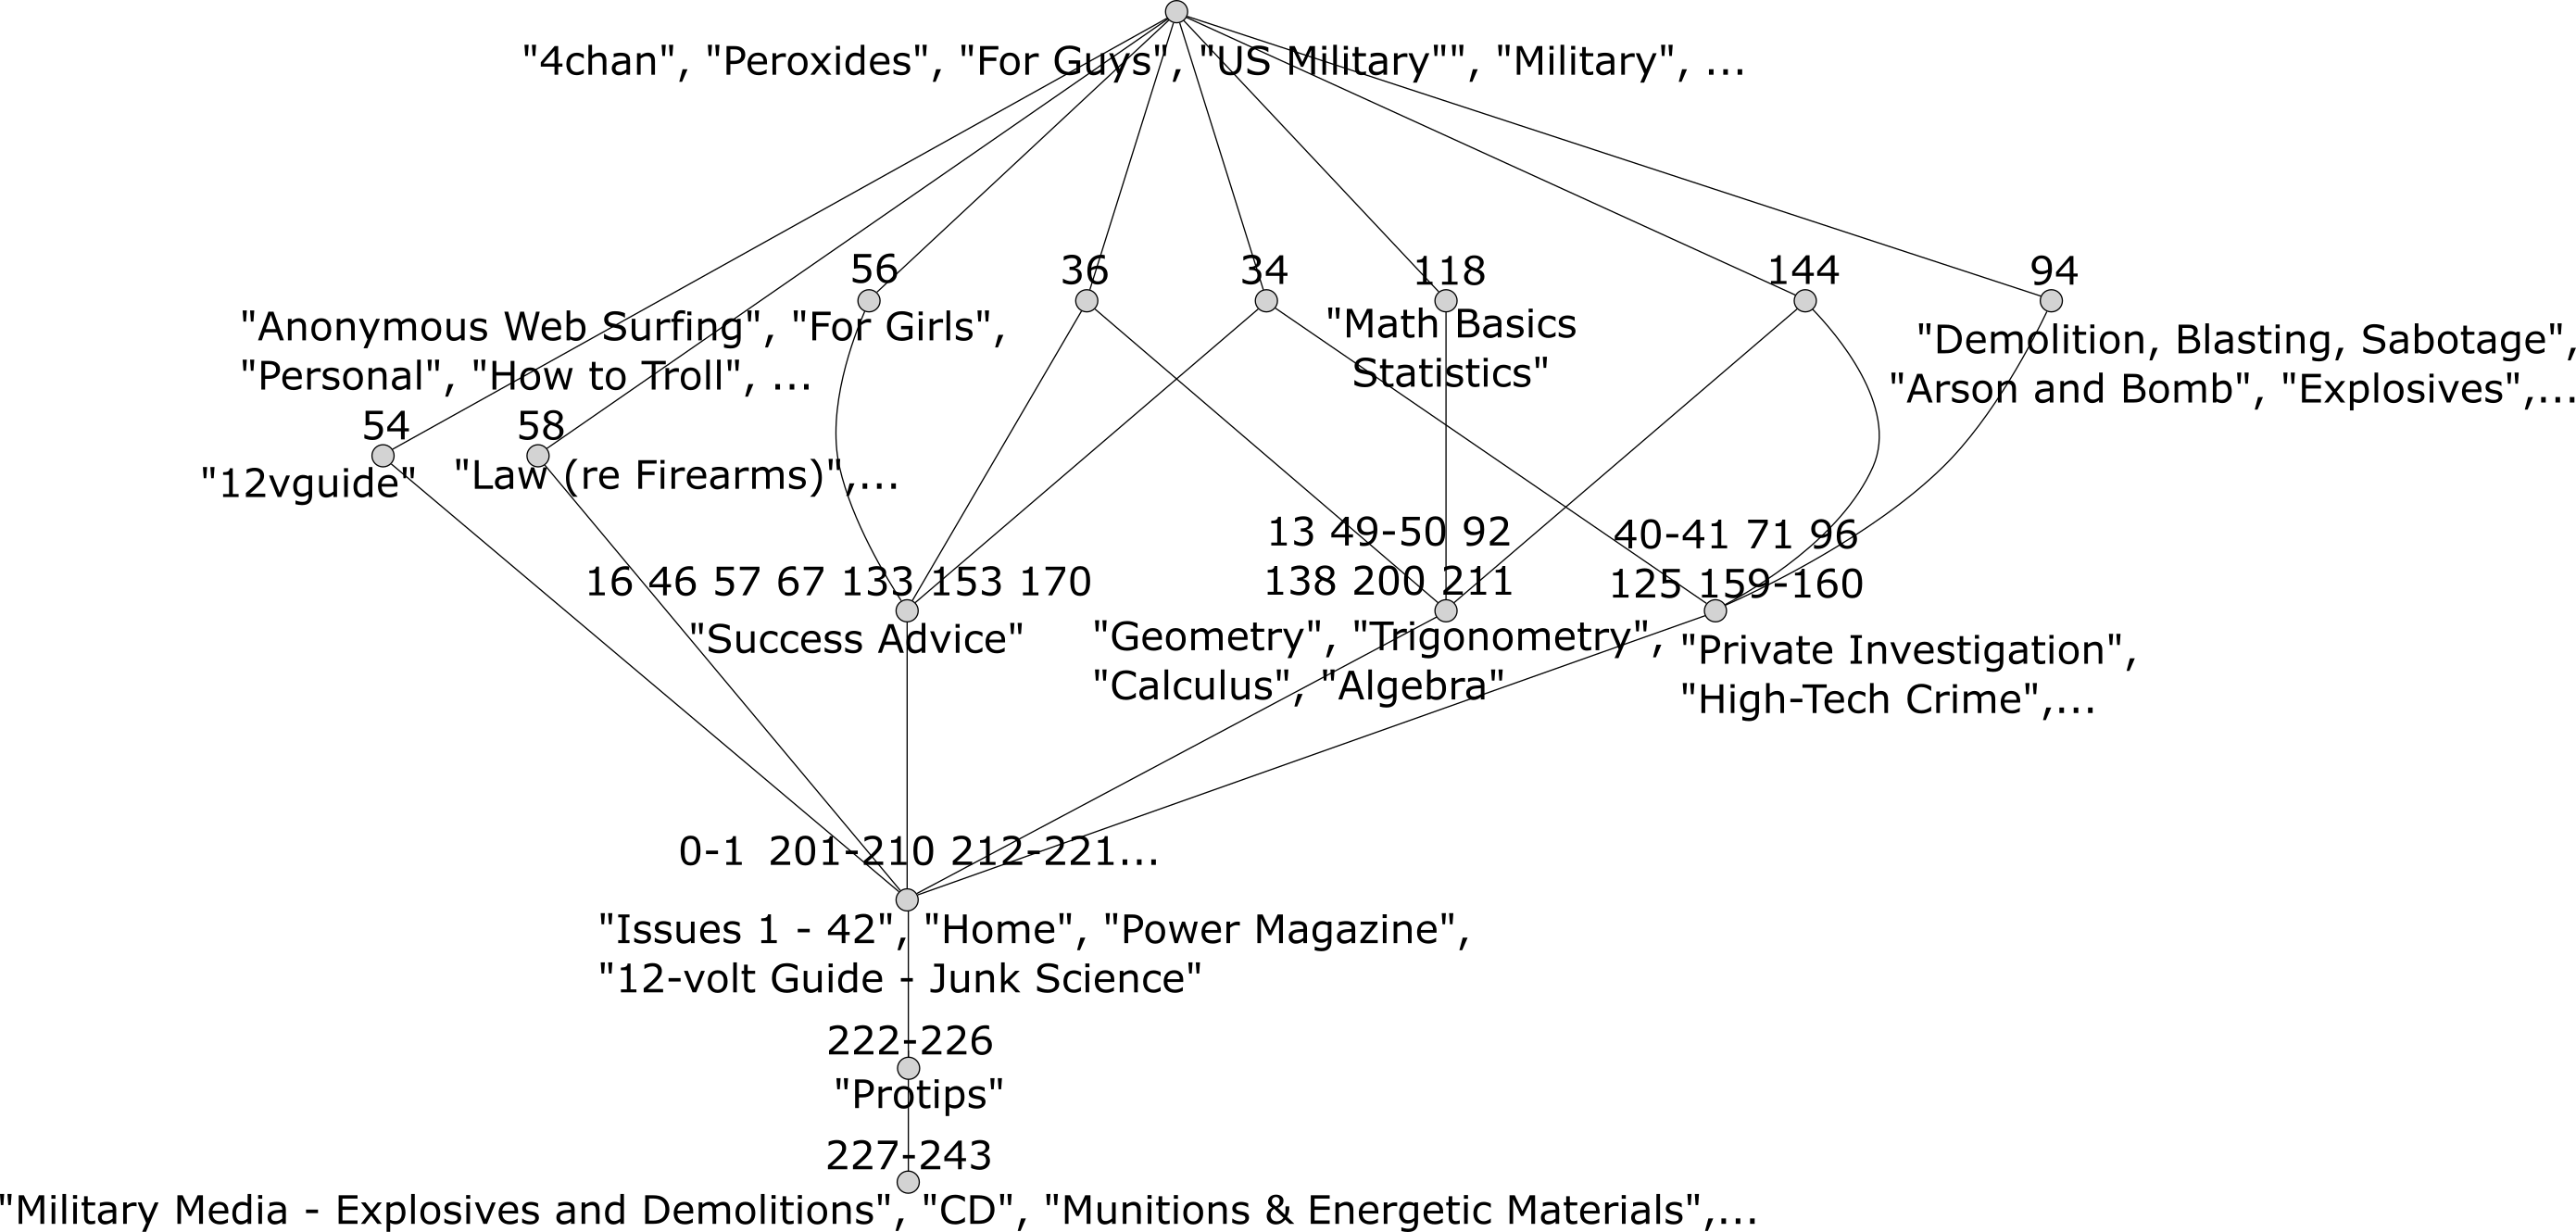
\includegraphics[width=0.7\textwidth]{images/fca_graph_across_dirs_02_03_25_reduced.png}
        \end{figure}
    }
    \only<5>{
        \begin{table}[H]
        \centering
        \resizebox{\textwidth}{!}{%
            \begin{tabular}{|
                    >{\columncolor[HTML]{D4D4D4}}l |l|l|l|l|l|}
                \hline
                \rowcolor[HTML]{D4D4D4}
                \textbf{Topic ID} & \multicolumn{5}{c|}{\textbf{Topic Words}}                                                                   \\ \hline
                \textbf{34}       & gun                                       & weapons      & rifles          & pistol         & firearm       \\ \hline
                \textbf{36}       & terminological                            & nonverbal    & linguist        & codeword       & longtext      \\ \hline
                \textbf{54}       & microelectron                             & microkernels & microparticle   & microphysics   & microcosmic   \\ \hline
                \textbf{56}       & pythonpath                                & pythonmac    & python\_version & python\_object & pythonpowered \\ \hline
                \textbf{58}       & nuclear                                   & hazardous    & explosive       & nanotoxicity   & chernobyl     \\ \hline
                \textbf{94}       & project                                   & fundraiser   & donation        & volunteering   & charity       \\ \hline
            \end{tabular}%
            }
        \end{table}
        }
    
    \vfill
    \visible<6->{
        \begin{center}
            {\color{myNewColorA}\LARGE Thank you for your attention!}
        \end{center}
    }
\end{frame}



\begin{frame}[allowframebreaks]
\frametitle{References}
\printbibliography
\end{frame}

\section*{List of abbreviations}

\begin{acronym}[XXXXXXXXX]
    \acro{fca}[FCA]{Formal Concept Analysis}
    \acro{dataset}[ETYNTKE]{Everything You Need To Know Ever}
    \acro{nlp}[NLP]{Natural Language Processing}
    \acro{git}[GIT]{Generative Image-to-text Transformer}
    \acro{pdf}[PDF]{Portable Document Format}
    \acro{ner}[NER]{Named Entity Recognition}
    \acro{ne}[NE]{Named Entity}
    \acro{sbert}[SBERT]{Sentence-BERT}
    \acro{use}[USE]{Universal Sentence Encoder}
    \acro{es}[ES]{Elasticsearch}
    \acro{umap}[UMAP]{Uniform Manifold Approximation and Projection for Dimension Reduction}
    \acro{tsne}[t-SNE]{t-Distributed Stochastic Neighbor Embedding}
    \acro{pca}[PCA]{Principal Component Analysis}
    \acro{hdbscan}[HDBSCAN]{Hierarchical Density-Based Spatial Clustering of Applications with Noise}
    \acro{bow}[BoW]{Bag of Words}
    \acro{tfidf}[TF-IDF]{Term Frequency-Inverse Document Frequency}
    \acro{approachname}[FAT-CAT]{FCA-based Aggregation for Topics using Conceptual Analysis and Taxonomies}
    \acro{cne}[CNE]{Clustering Named Entities}
    \acro{edr}[EDR]{Embedding - Dimension Reduction}
    \acro{hlda}[hLDA]{Hierarchical Latent Dirichlet Allocation}

    % \acro{}[]{}
\end{acronym}
\appendix
\section{Supplementary Material}

\begin{frame}{Image Captioner~\cite{git_2022}}
    \label{supp:img_cap}
    \begin{figure}
        \includesvg[width=\linewidth]{images/git_image_captioner}
        \caption{\ac{git}\footnote{\url{https://huggingface.co/microsoft/git-base} (29.01.2025)}}
    \end{figure}
\end{frame}

\begin{frame}{\ac{sbert}~\cite{sbert_2019}}
    \label{supp:sbert}
    \includesvg[width=\linewidth]{images/SentenceBERT}
\end{frame}

\begin{frame}{\ac{use}~\cite{use_2019}}
    \label{supp:use}
    \includesvg[width=\linewidth]{images/USE}
\end{frame}
\end{document}



